\chapter{Drawings}

Using package TikZ we will get a drawing instead of using Paint.


\section{Tank equation}
\begin{figure}[h]
    \centering
    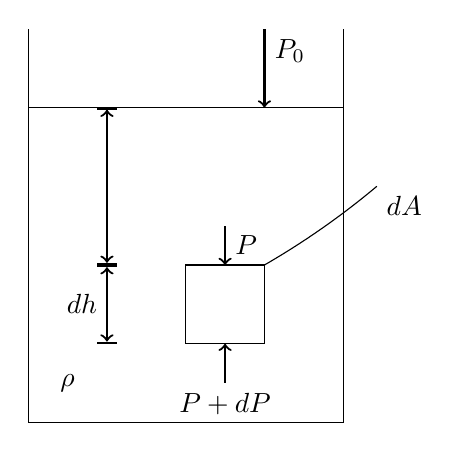
\begin{tikzpicture}
    \draw (0,0) rectangle (4,4);
    \draw (0,4) -- (0,5);
    \draw (4,4) -- (4,5);
    \draw[thick, <-] (3,4) -- (3,5) node[anchor=north west]{$P_0$};
    \draw (2,1) rectangle (3,2);
    \draw[thick, <-] (2.5,2) -- (2.5,2.5) node[anchor=north west]{$P$};
    \draw[thick, <-] (2.5,1) -- (2.5,0.5) node[anchor= north]{$P+dP$};
    \draw (0.5,0.5) node{$\rho$};
    \draw (3,2) arc (300:310:10cm) node[anchor=north west]{$dA$};
    \draw[thick, |<->|] (1,4) -- (1,2);
    \draw[thick, |<->|] (1,2) -- (1,1);
    \draw (1,1.5) node[anchor=east]{$dh$};
    \end{tikzpicture}
    \caption{Tank and pressure}
    \label{fig:tank}
\end{figure}

\newpage
\section{Ultrasound on objects}
\begin{figure}[h]
    \centering
    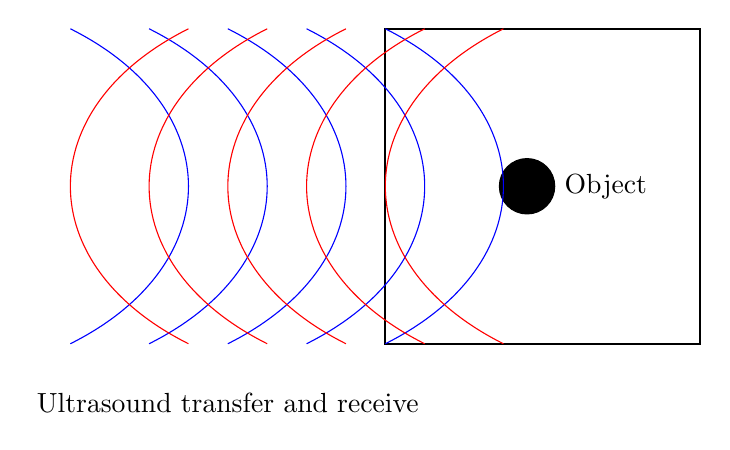
\begin{tikzpicture}
    \filldraw[color=black] (-2.2,0) circle (10pt) node[xshift=1cm] {Object};
    \draw[thick] (-4,-2) rectangle (0,2);
    \foreach \x in {4,5,6,7,8}
        \draw[color=blue] (-\x,2) .. controls (-\x+2,1) and (-\x+2,-1) .. (-\x,-2);
    \foreach \x in {2.5,3.5,4.5,5.5,6.5}
        \draw[color=red] (-\x,2) .. controls (-\x-2,1) and (-\x-2,-1) .. (-\x,-2);
    \draw (-6,-2.5) node[anchor=north] {Ultrasound transfer and receive};
    \end{tikzpicture}
    \caption{Ultrasound}
    \label{fig:Ultrasound}
\end{figure}

\newpage
\section{Control volumes}
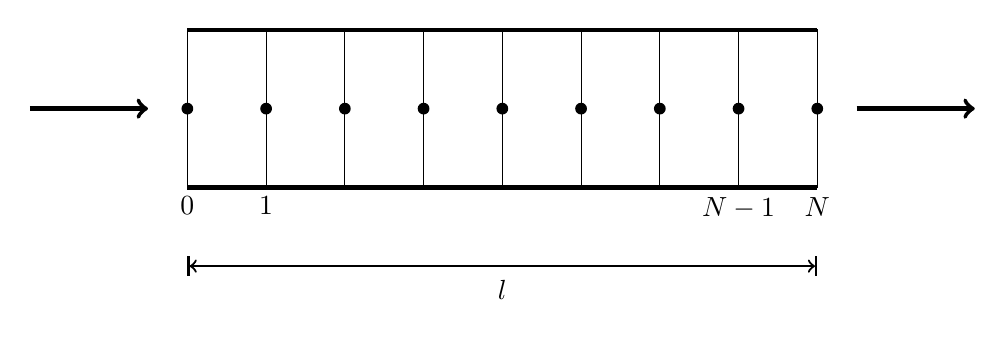
\begin{tikzpicture}
\foreach \x in {0,1}
   \draw (\x+2,2) rectangle (\x, 0) node[anchor=north] {$\x$};
\foreach \y in {2,3,4,5}   
   \draw (\y+2,2) rectangle (\y, 0);
\draw (7,2) rectangle (8,0) node[anchor=north] {$N$};
\draw (7,0) node[anchor=north] {$N-1$};
\draw[ultra thick] (0,0) -- (8,0);
\draw[ultra thick] (0,2) -- (8,2);
\draw[|<->|,thick] (0,-1) -- (8,-1) node[pos=0.5, yshift=-0.3cm]{$l$};
\draw[->, ultra thick] (-2,1) -- (-0.5,1);
\draw[->, ultra thick] (8.5,1) -- (10,1);
\foreach \n in {0,1,2,3,4,5,6,7,8}
  \node at (\n,1)[circle,fill,inner sep=1.5pt]{};
\end{tikzpicture}

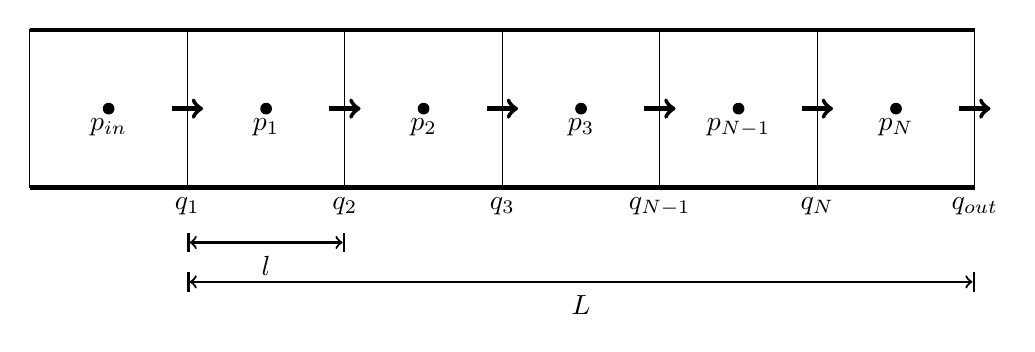
\begin{tikzpicture}
\foreach \x in {1,2,3}
   \draw (2*\x,2) rectangle (2*\x-2, 0) node[anchor=north] {$q_{\x}$};
\draw (8,2) rectangle (6, 0) node[anchor=north] {$q_{N-1}$};
\draw (10,2) rectangle (8, 0) node[anchor=north] {$q_{N}$};
\draw (8,2) rectangle (10,0) node[anchor=north] {$q_{out}$};
\draw (-2,2) rectangle (0,0);
\draw (-1,1) node[anchor=north] {$p_{in}$};
\draw[ultra thick] (-2,0) -- (10,0);
\draw[ultra thick] (-2,2) -- (10,2);
\draw[|<->|,thick] (0,-1.2) -- (10,-1.2) node[pos=0.5, yshift=-0.3cm]{$L$};
\draw[|<->|,thick] (0,-0.7) -- (2,-0.7) node[pos=0.5, yshift=-0.3cm]{$l$};
\foreach \n in {-1,1,3,5,7,9}
    \node at (\n,1)[circle,fill,inner sep=1.5pt]{};
\foreach \m in {1,2,3}
    \draw (2*\m-1,1) node[anchor=north] {$p_{\m}$};
\draw (7,1) node[anchor=north] {$p_{N-1}$};
\draw (9,1) node[anchor=north] {$p_{N}$};
\foreach \o in {0,2,4,6,8,10}
    \draw[->, ultra thick] (\o-0.2,1) -- (\o+0.2,1);
\end{tikzpicture}


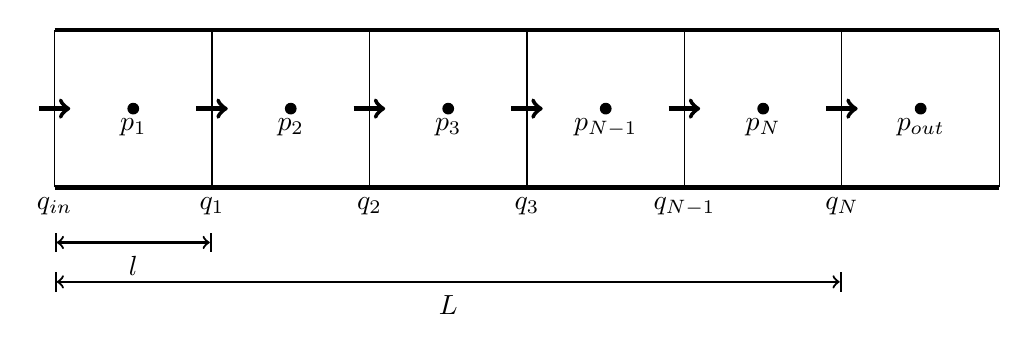
\begin{tikzpicture}
\foreach \x in {1,2,3}
   \draw (2*\x,2) rectangle (2*\x, 0) node[anchor=north] {$q_{\x}$};
\draw (8,2) rectangle (8, 0) node[anchor=north] {$q_{N-1}$};
\draw (10,2) rectangle (10, 0) node[anchor=north] {$q_{N}$};
\draw (0,0) node[anchor=north] {$q_{in}$};
\draw[ultra thick] (0,0) -- (12,0);
\draw[ultra thick] (0,2) -- (12,2);
\draw (11,1) node[anchor=north] {$p_{out}$};
\draw (0,0) -- (0,2);
\draw (12,0) -- (12,2);
\draw[|<->|,thick] (0,-1.2) -- (10,-1.2) node[pos=0.5, yshift=-0.3cm]{$L$};
\draw[|<->|,thick] (0,-0.7) -- (2,-0.7) node[pos=0.5, yshift=-0.3cm]{$l$};
\foreach \n in {1,3,5,7,9,11}
    \node at (\n,1)[circle,fill,inner sep=1.5pt]{};
\foreach \m in {1,2,3}
    \draw (2*\m-1,1) node[anchor=north] {$p_{\m}$};
\foreach \o in {0,2,4,6,8,10}
    \draw[->, ultra thick] (\o-0.2,1) -- (\o+0.2,1);
\draw (7,1) node[anchor=north] {$p_{N-1}$};
\draw (9,1) node[anchor=north] {$p_{N}$};
\end{tikzpicture}

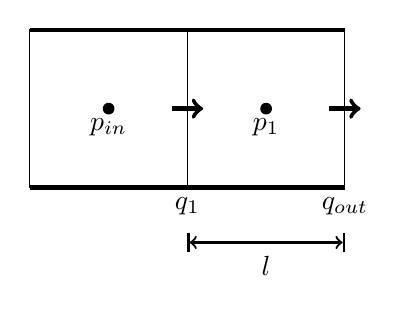
\begin{tikzpicture}
\draw (0,2) rectangle (2, 0) node[anchor=north] {$q_{out}$};
\draw (0,2) rectangle (-2, 0);
\draw (0,0) node[anchor=north] {$q_{1}$};
\draw (-1,1) node[anchor=north] {$p_{in}$};
\draw[ultra thick] (-2,0) -- (2,0);
\draw[ultra thick] (-2,2) -- (2,2);
\draw[|<->|,thick] (0,-0.7) -- (2,-0.7) node[pos=0.5, yshift=-0.3cm]{$l$};
\foreach \n in {0,1}
    \node at (2*\n-1,1)[circle,fill,inner sep=1.5pt]{};
\foreach \m in {1}
    \draw (2*\m-1,1) node[anchor=north] {$p_{\m}$};
\foreach \o in {0,2}
    \draw[->, ultra thick] (\o-0.2,1) -- (\o+0.2,1);
\end{tikzpicture}


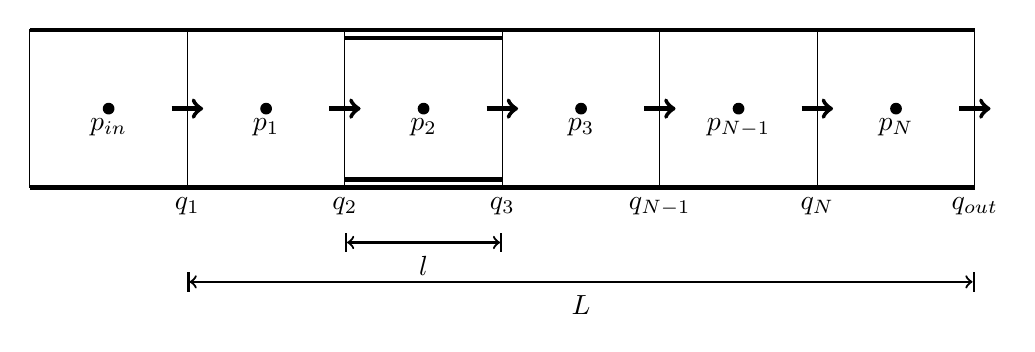
\begin{tikzpicture}
\foreach \x in {1,2,3}
   \draw (2*\x,2) rectangle (2*\x-2, 0) node[anchor=north] {$q_{\x}$};
\draw (8,2) rectangle (6, 0) node[anchor=north] {$q_{N-1}$};
\draw (10,2) rectangle (8, 0) node[anchor=north] {$q_{N}$};
\draw (8,2) rectangle (10,0) node[anchor=north] {$q_{out}$};
\draw (-2,2) rectangle (0,0);
\draw (-1,1) node[anchor=north] {$p_{in}$};
\draw[ultra thick] (-2,0) -- (10,0);
\draw[ultra thick] (-2,2) -- (10,2);
\draw[ultra thick] (4,0.1) -- (2,0.1);
\draw[ultra thick] (4,1.9) -- (2,1.9);
\draw[|<->|,thick] (0,-1.2) -- (10,-1.2) node[pos=0.5, yshift=-0.3cm]{$L$};
\draw[|<->|,thick] (4,-0.7) -- (2,-0.7) node[pos=0.5, yshift=-0.3cm]{$l$};
\foreach \n in {-1,1,3,5,7,9}
    \node at (\n,1)[circle,fill,inner sep=1.5pt]{};
\foreach \m in {1,2,3}
    \draw (2*\m-1,1) node[anchor=north] {$p_{\m}$};
\draw (7,1) node[anchor=north] {$p_{N-1}$};
\draw (9,1) node[anchor=north] {$p_{N}$};
\foreach \o in {0,2,4,6,8,10}
    \draw[->, ultra thick] (\o-0.2,1) -- (\o+0.2,1);
\end{tikzpicture}


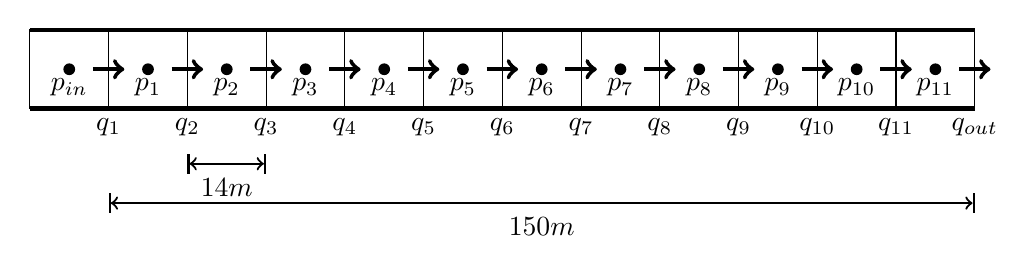
\begin{tikzpicture}
\foreach \x in {1,2,3,4,5,6,7,8,9,10,11}
   \draw (1*\x,1) rectangle (\x-1, 0) node[anchor=north] {$q_{\x}$};
\draw (10,1) rectangle (11,0) node[anchor=north] {$q_{out}$};
\draw (-1,1) rectangle (0,0);
\draw (-0.5,0.5) node[anchor=north] {$p_{in}$};
\draw[ultra thick] (-1,0) -- (11,0);
\draw[ultra thick] (-1,1) -- (11,1);
\draw[|<->|,thick] (0,-1.2) -- (11,-1.2) node[pos=0.5, yshift=-0.3cm]{$150 m$};
\draw[|<->|,thick] (1,-0.7) -- (2,-0.7) node[pos=0.5, yshift=-0.3cm]{$14 m$};
\foreach \n in {0,1,2,3,4,5,6,7,8,9,10,11}
    \node at (\n-0.5,0.5)[circle,fill,inner sep=1.5pt]{};
\foreach \m in {1,2,3,4,5,6,7,8,9,10,11}    
    \draw (\m-0.5,0.5) node[anchor=north] {$p_{\m}$};
\foreach \o in {0,1,2,3,4,5,6,7,8,9,10,11}
    \draw[->, ultra thick] (\o-0.2,0.5) -- (\o+0.2,0.5);
\end{tikzpicture}



